% !TEX root = template.tex

\section{Results}
\label{sec:results}

As in most of the works mentioned in section \ref{sec:related_work}, besides accuracy, we used $F_1$ measure to estimate the goodness of our models. Defining precision and recall as: 
\begin{equation}
	p = \frac{TP}{TP+FP} \qquad r = \frac{TP}{TP+FN}
\end{equation}
the $F_1$ measure is evaluated as the harmonic average between the two (in the previous formula we have \textit{TP = true positive}, \textit{FP = false positive}, \textit{FN = false negative}). In particular, since we deal with a multi-class problem we need to add a measure of weights to the $F_1$ equation:
\begin{equation}
	F_1 = \sum_i 2w_i \frac{p_i \cdot r_i}{p_i + r_i}
\end{equation} 
where the weights are defined as the number of samples of a particular class divided by the total number of samples $w_i = \frac{n_i}{N}$. The weighted measure can help also with the class imbalance problem that we outlined in the previous section; we must highlight however that our models are still trained on an imbalanced dataset, so in our opinion this could provide only a minor improvement.

In Figures \ref{fig:Anull} and \ref{fig:Anonull} we present the results regarding task A (modes of locomotion, high level movements) for each participant of the experiment: in those configurations we wanted to see if there was one architecture that evidently outperform the others. As we can see, unfortunately that is not the case since among all the frameworks that we tested the differences in terms of weighted $F_1$ measure is negligible. The variation that we can clearly see is among distinct subjects, since they are all studied separately: $S_1$ for example performs better in both the configurations, while $S_2$ is typically the worst. Considering that we consistently performed the same procedure independently from the subject, in this case this discrepancy could be due to a problem occurred during data collection. 

\begin{figure}[ht]
	\centering
	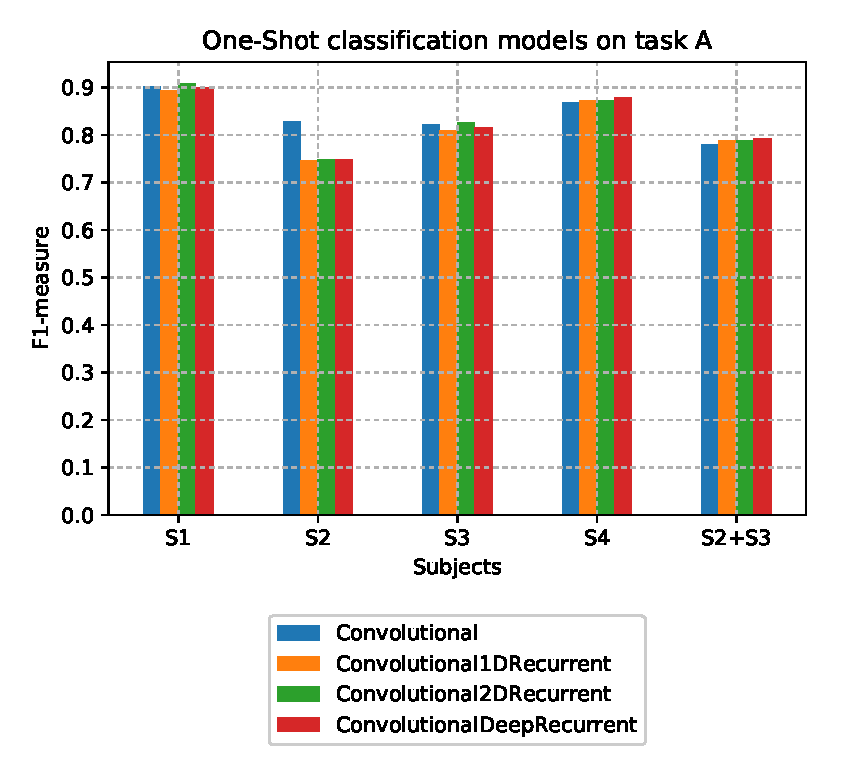
\includegraphics[scale=.4]{figure/A_models_nullclass}
	\caption{Task A : One-Shot Classification}
	\label{fig:Anull}
\end{figure}

With an $F_1$ value of $\sim 0.91$ for the \textit{one-shot} scenario and $\sim 0.94$ in the \textit{two-steps} (if we just consider $S_1$), we can definitely say that the results presented in \cite{Chavarriaga2013} are outperformed by these more powerful deep learning models; with respect to the other subjects, we can say that we obtained state of the art results. In particular it's interesting to see that, when we consider the \textit{Null Class}, the best model with $S_2$ is represented by the neural network with one convolutional layer (Figure \ref{fig:Anull}); when the \textit{Null Class} is discarded, instead, the hybrid model that combines convolutional layers and LSTM provides the best results (Figure \ref{fig:Anonull}). In our opinion the reason is that in certain cases the \textit{Null Class} has to be intended as noise so, when the windows assigned to that class are removed, the LSTM can exploit and reveal the time correlation among different samples more clearly. In addition, we tried to train our architectures on $S_2$ and $S_3$ jointly, using $ADL_4$ and $ADL_5$ of both subjects as test set: as is shown on the last column on the right in Fig \ref{fig:Anull} and \ref{fig:Anonull}, the results are not brilliant. In fact, we obtained a kind of average performance between the results of $S_2$ and $S_3$, in line again with what presented in \cite{Chavarriaga2013}. Finally, as we can see, for task A the use of the \textit{two-step} approach definitely improved performances for all users. 

\begin{figure}[ht]
	\centering
	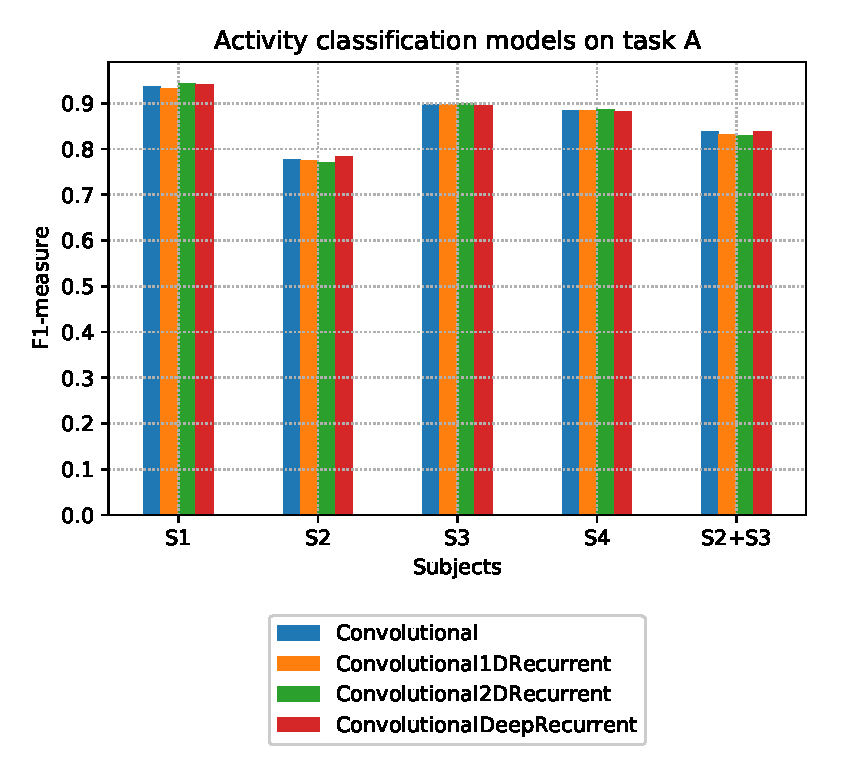
\includegraphics[scale=.4]{figure/A_models_nonullclass}
	\caption{Task A : Two Steps Classification}
	\label{fig:Anonull}
\end{figure}

Despite the promising results on high-level movement classification, when we used our models to do the more precise and low-level classification of task B, the \textit{two-steps} configuration wasn't effective as we hoped - Figure \ref{fig:Bnonull}. Still, in both architectures $S_2$ is the one that performs the worst, while with $S_1$ we are able to extract the best results; moreover, even in this case we haven't noticed considerable differences among the different neural network set-ups that we used: this suggests us, as we briefly outlined in previous sections, increasing the complexity of the architecture in order to obtain astonishing results, isn't the right path to follow. 

We can see in Figure \ref{fig:Bnull} that implementing one convolutional layer jointly with 2 LSTM followed by 2 fully connected layers, contributed positively on the performances of \textit{one-shot} model, for all subjects considered. The considerations done for Task A, regarding the behaviour of the models fed with $S_1$ and $S_2$ together, remains valid also for Task B. 

\begin{figure}[ht]
	\centering
	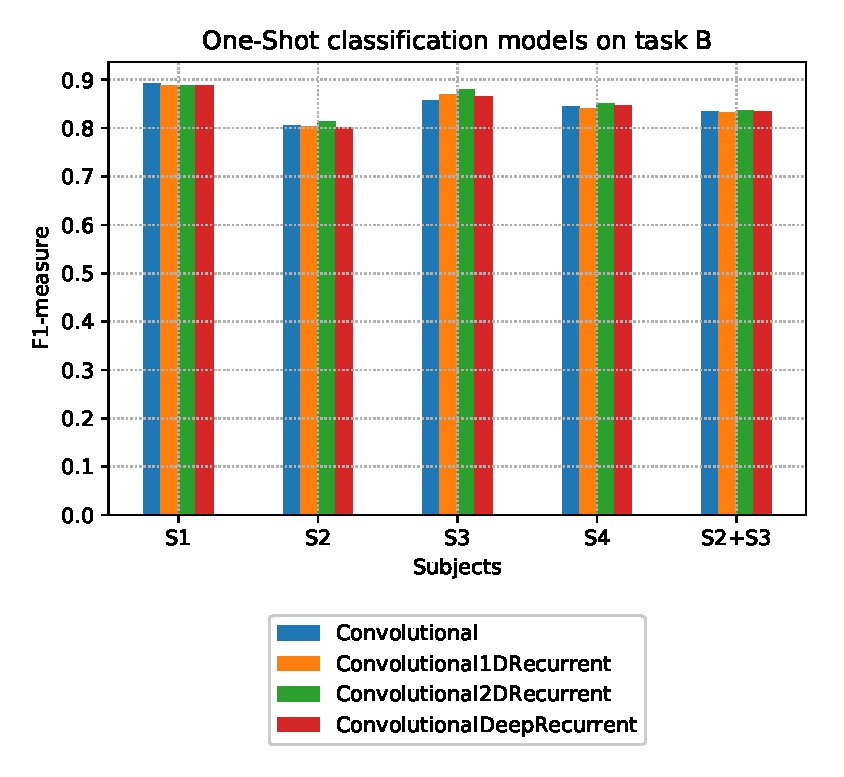
\includegraphics[scale=.4]{figure/B_models_nullclass}
	\caption{Task B : One-Shot Classification}
	\label{fig:Bnull}
\end{figure}

In general however, despite $S_2$, the results for the configuration in Figure \ref{fig:Bnonull} are better with respect to what presented by Chavarriaga in \cite{Chavarriaga2013}; regarding what shown in Figure \ref{fig:Bnull} we can say that the results are compatible with the state of art, reaching a value of $\sim 90\%$ for $S_1$. 

In conclusion we found out that, even with powerful deep learning models, if we discard the \textit{Null Class} the results are not appealing when we have to deal with many classes (in addition, affected by the imbalance problem); this, however, shouldn't discourage researchers to go down this path. Considering that for Task B we reached almost $\sim 0.92$ in the detection step for $S_1$, this suggests us that building two distinct models for detection and classification respectively could lead to promising results: the design of a specific model for each step could focus the effort on a single purpose, in this way leading to ad-hoc and less complex networks. In our work however we wanted to see how the problem could be tackled with the solutions proposed by the state of the art, still trying to reduce computational effort. Just to make some numeric comparison, while the Hybrid model proposed in \cite{HAR-COMP2018} counts 17 millions of trainable parameters, our most complex model reduced this number more than an half. 

\begin{figure}[ht]
	\centering
	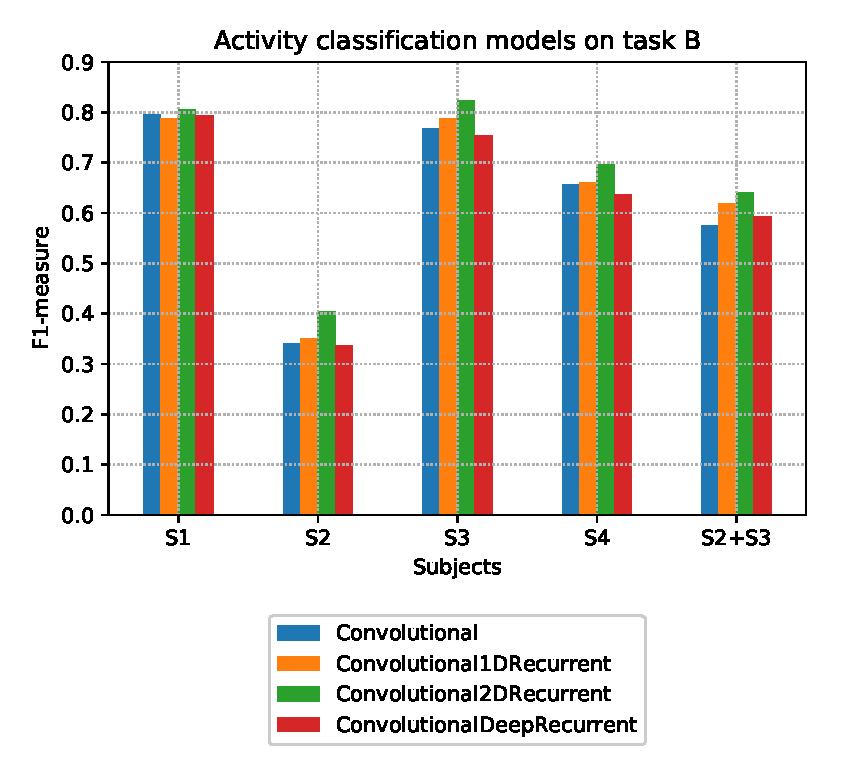
\includegraphics[scale=.4]{figure/B_models_nonullclass}
	\caption{Task B : Two Steps Classification}
	\label{fig:Bnonull}
\end{figure}